% Drawing 8/03-1 -- folder 8, batch 03, archive page 57 (PDF page 58).
% Transcription: feuillet quadrillé tenu en largeur, au crayon. En haut à gauche, sous « $n/17$ », sept petites lignes brisées, une par ligne (« $n = 1, 2, 3$ », « $n = 4$ », « $n = 5$ », « $n = 6$ », « $n = 7, \dots, 13$ », « $n = 14$ », « $n = 15, 16$ »), et la colonne « $\nu$ » : $1, 2, 3, 1, 2, 3, 2$. Au centre, un axe horizontal gradué de 1 à 18 et, à son extrémité droite, un axe vertical gradué de 1 à 16 ; deux longues droites presque parallèles montent de la gauche de l'axe jusqu'au coin supérieur droit, des points marqués le long ; à droite, un faisceau de seize segments de pentes décroissantes aboutit aux seize graduations de l'axe vertical.
% Kind: whole-page pencil graph on squared paper (lines of slope n/17, small broken lines). Method 2 (schematic redraw from the facsimile). Status: partial.
% Notes: Whole page, faint pencil on squared paper held lengthwise. Drawn: the horizontal axis with its graduations 1 to 18 and the vertical axis at abscissa 18 with its graduations 1 to 16, both on a computed lattice (one square = 3.6 units); the two long nearly parallel lines from the left end of the axis to the upper right corner; eight marked points along them; the fan at the right, drawn as the right-hand ends of the sixteen lines from the origin to the points (18, n), n = 1, ..., 16, each over the length seen on the page (a reading: on the page the segments point towards the origin and end on the sixteen graduations); at the top left the seven small broken lines with their labels n = ..., the heading n/17 and the column headed nu (1, 2, 3, 1, 2, 3, 2). Left out: the inequalities between fractions written all round the graph (they are in the transcription), « 2533 > 285 », the scribble at the top right, the ruling of the paper, further faint lattice dots in the middle of the sheet and the faint doublings of several segments of the fan. Still differs: the small broken lines are read off a 200 dpi render and approximate; the lengths of the fan segments are approximate; the two long lines are placed by their ends only. Redrawn 2026-11-12 (issue 128): to check again.
% Coordinates: 1 unit = 1 mm = 1/100 of the crop width (bbox in page fractions: [0.09, 0.068, 1.0, 0.565]).
% Redrawn by Claude (claude-fable-5-2), issue #128, 2026-11-12; not checked by a human; not compiled (no TeX in the session).
% Rights: reproduces part of the work -- behind RENDER_TRANSCRIPTS, never published by itself.
\documentclass[tikz,border=3pt]{standalone}
\usepackage{amsmath,amssymb}
\usetikzlibrary{patterns,arrows.meta}
\tikzset{pencil/.style={black!45}, struck/.style={black!35}, mpt/.style={circle,draw,inner sep=1.3pt}, pt/.style={circle,fill,inner sep=0.9pt}, opt/.style={circle,draw,fill=white,inner sep=1.1pt}}
\begin{document}
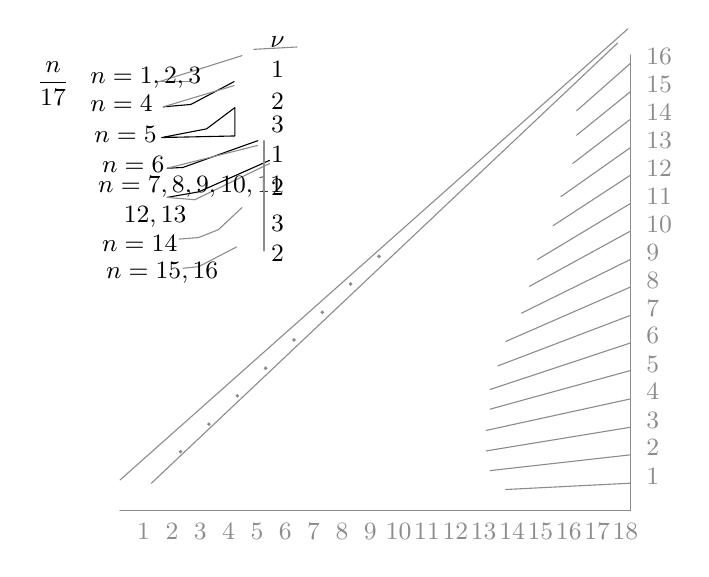
\begin{tikzpicture}[x=1mm,y=1mm,line cap=round,line join=round,font=\small]
\draw[pencil] (17,-62) -- (81.8,-62);
\draw[pencil] (81.8,-62) -- (81.8,-4.1);
\node[pencil] at (20,-64.6) {\small $1$};
\node[pencil] at (23.6,-64.6) {\small $2$};
\node[pencil] at (27.2,-64.6) {\small $3$};
\node[pencil] at (30.8,-64.6) {\small $4$};
\node[pencil] at (34.4,-64.6) {\small $5$};
\node[pencil] at (38,-64.6) {\small $6$};
\node[pencil] at (41.6,-64.6) {\small $7$};
\node[pencil] at (45.2,-64.6) {\small $8$};
\node[pencil] at (48.8,-64.6) {\small $9$};
\node[pencil] at (52.4,-64.6) {\small $10$};
\node[pencil] at (56,-64.6) {\small $11$};
\node[pencil] at (59.6,-64.6) {\small $12$};
\node[pencil] at (63.2,-64.6) {\small $13$};
\node[pencil] at (66.8,-64.6) {\small $14$};
\node[pencil] at (70.4,-64.6) {\small $15$};
\node[pencil] at (74,-64.6) {\small $16$};
\node[pencil] at (77.6,-64.6) {\small $17$};
\node[pencil] at (81.2,-64.6) {\small $18$};
\node[pencil,right] at (82.6,-57.6) {\small $1$};
\node[pencil,right] at (82.6,-54) {\small $2$};
\node[pencil,right] at (82.6,-50.5) {\small $3$};
\node[pencil,right] at (82.6,-46.9) {\small $4$};
\node[pencil,right] at (82.6,-43.4) {\small $5$};
\node[pencil,right] at (82.6,-39.8) {\small $6$};
\node[pencil,right] at (82.6,-36.3) {\small $7$};
\node[pencil,right] at (82.6,-32.7) {\small $8$};
\node[pencil,right] at (82.6,-29.2) {\small $9$};
\node[pencil,right] at (82.6,-25.6) {\small $10$};
\node[pencil,right] at (82.6,-22.1) {\small $11$};
\node[pencil,right] at (82.6,-18.5) {\small $12$};
\node[pencil,right] at (82.6,-15) {\small $13$};
\node[pencil,right] at (82.6,-11.4) {\small $14$};
\node[pencil,right] at (82.6,-7.8) {\small $15$};
\node[pencil,right] at (82.6,-4.3) {\small $16$};
\draw[pencil] (17,-58.1) -- (81.5,-0.8);
\draw[pencil] (21,-58.5) -- (80.2,-2.6);
\node[pt,pencil,inner sep=0.5pt] at (24.7,-54.5) {};
\node[pt,pencil,inner sep=0.5pt] at (28.3,-51) {};
\node[pt,pencil,inner sep=0.5pt] at (31.9,-47.4) {};
\node[pt,pencil,inner sep=0.5pt] at (35.5,-43.9) {};
\node[pt,pencil,inner sep=0.5pt] at (39.1,-40.3) {};
\node[pt,pencil,inner sep=0.5pt] at (42.7,-36.8) {};
\node[pt,pencil,inner sep=0.5pt] at (46.3,-33.2) {};
\node[pt,pencil,inner sep=0.5pt] at (49.9,-29.7) {};
\draw[pencil] (66,-59.3) -- (81.8,-58.5);
\draw[pencil] (64,-56.9) -- (81.8,-54.9);
\draw[pencil] (63.5,-54.4) -- (81.8,-51.4);
\draw[pencil] (63.5,-51.8) -- (81.8,-47.8);
\draw[pencil] (64,-49.1) -- (81.8,-44.2);
\draw[pencil] (64,-46.6) -- (81.8,-40.7);
\draw[pencil] (65,-43.6) -- (81.8,-37.2);
\draw[pencil] (66,-40.5) -- (81.8,-33.6);
\draw[pencil] (68,-36.9) -- (81.8,-30.1);
\draw[pencil] (69,-33.5) -- (81.8,-26.5);
\draw[pencil] (70,-30.1) -- (81.8,-23);
\draw[pencil] (72,-25.8) -- (81.8,-19.4);
\draw[pencil] (73,-22.1) -- (81.8,-15.9);
\draw[pencil] (74.5,-17.9) -- (81.8,-12.3);
\draw[pencil] (75,-14.3) -- (81.8,-8.8);
\draw[pencil] (75,-11.2) -- (81.8,-5.2);
\draw[pencil] (21.5,-7.5) -- (26,-7.5);
\draw[pencil] (22,-7.5) -- (32.5,-4.2);
\draw (22.5,-10.7) -- (26,-10.4) -- (31.5,-7.5);
\draw[pencil] (22.5,-10.7) -- (31.5,-8);
\draw (22.3,-14.6) -- (28,-13.5) -- (31.6,-10.8) -- (31.6,-14.4) -- cycle;
\draw (23,-18.5) -- (25,-18.4) -- (34.5,-15);
\draw[pencil] (23,-18.5) -- (34.5,-15.6);
\draw (23,-22.2) -- (27,-21.5) -- (36,-17.5);
\draw[pencil] (23,-22.2) -- (26.5,-22.5) -- (36,-17.9);
\draw[pencil] (24.5,-27.5) -- (27,-27.3) -- (29.5,-26.3) -- (32.5,-23.5);
\draw[pencil] (25,-31.2) -- (27,-31) -- (31.8,-28.5);
\node at (8.5,-7.8) {\small $\dfrac{n}{17}$};
\node[right] at (12,-7) {\small $n = 1, 2, 3$};
\node[right] at (12,-10.3) {\small $n = 4$};
\node[right] at (12.5,-14.2) {\small $n = 5$};
\node[right] at (13.5,-18) {\small $n = 6$};
\node[right,align=left] at (13,-22.8) {\small $n = 7, 8, 9, 10, 11$\\\small $\quad 12, 13$};
\node[right] at (13.5,-28) {\small $n = 14$};
\node[right] at (14,-31.8) {\small $n = 15, 16$};
\node at (37,-2.5) {\small $\nu$};
\draw[pencil] (34,-3.4) -- (39.5,-3.1);
\draw[pencil] (35.3,-15) -- (35.3,-29);
\node at (37,-6) {\small $1$};
\node at (37,-10) {\small $2$};
\node at (37,-13) {\small $3$};
\node at (37,-16.7) {\small $1$};
\node at (37,-21) {\small $2$};
\node at (37,-25.5) {\small $3$};
\node at (37,-29.3) {\small $2$};
\end{tikzpicture}
\end{document}
